\documentclass[12pt,english,french]{report}\usepackage{graphicx, color}
%% maxwidth is the original width if it is less than linewidth
%% otherwise use linewidth (to make sure the graphics do not exceed the margin)
\makeatletter
\def\maxwidth{ %
  \ifdim\Gin@nat@width>\linewidth
    \linewidth
  \else
    \Gin@nat@width
  \fi
}
\makeatother

\definecolor{fgcolor}{rgb}{0.2, 0.2, 0.2}
\newcommand{\hlnumber}[1]{\textcolor[rgb]{0,0,0}{#1}}%
\newcommand{\hlfunctioncall}[1]{\textcolor[rgb]{0.501960784313725,0,0.329411764705882}{\textbf{#1}}}%
\newcommand{\hlstring}[1]{\textcolor[rgb]{0.6,0.6,1}{#1}}%
\newcommand{\hlkeyword}[1]{\textcolor[rgb]{0,0,0}{\textbf{#1}}}%
\newcommand{\hlargument}[1]{\textcolor[rgb]{0.690196078431373,0.250980392156863,0.0196078431372549}{#1}}%
\newcommand{\hlcomment}[1]{\textcolor[rgb]{0.180392156862745,0.6,0.341176470588235}{#1}}%
\newcommand{\hlroxygencomment}[1]{\textcolor[rgb]{0.43921568627451,0.47843137254902,0.701960784313725}{#1}}%
\newcommand{\hlformalargs}[1]{\textcolor[rgb]{0.690196078431373,0.250980392156863,0.0196078431372549}{#1}}%
\newcommand{\hleqformalargs}[1]{\textcolor[rgb]{0.690196078431373,0.250980392156863,0.0196078431372549}{#1}}%
\newcommand{\hlassignement}[1]{\textcolor[rgb]{0,0,0}{\textbf{#1}}}%
\newcommand{\hlpackage}[1]{\textcolor[rgb]{0.588235294117647,0.709803921568627,0.145098039215686}{#1}}%
\newcommand{\hlslot}[1]{\textit{#1}}%
\newcommand{\hlsymbol}[1]{\textcolor[rgb]{0,0,0}{#1}}%
\newcommand{\hlprompt}[1]{\textcolor[rgb]{0.2,0.2,0.2}{#1}}%

\usepackage{framed}
\makeatletter
\newenvironment{kframe}{%
 \def\at@end@of@kframe{}%
 \ifinner\ifhmode%
  \def\at@end@of@kframe{\end{minipage}}%
  \begin{minipage}{\columnwidth}%
 \fi\fi%
 \def\FrameCommand##1{\hskip\@totalleftmargin \hskip-\fboxsep
 \colorbox{shadecolor}{##1}\hskip-\fboxsep
     % There is no \\@totalrightmargin, so:
     \hskip-\linewidth \hskip-\@totalleftmargin \hskip\columnwidth}%
 \MakeFramed {\advance\hsize-\width
   \@totalleftmargin\z@ \linewidth\hsize
   \@setminipage}}%
 {\par\unskip\endMakeFramed%
 \at@end@of@kframe}
\makeatother

\definecolor{shadecolor}{rgb}{.97, .97, .97}
\definecolor{messagecolor}{rgb}{0, 0, 0}
\definecolor{warningcolor}{rgb}{1, 0, 1}
\definecolor{errorcolor}{rgb}{1, 0, 0}
\newenvironment{knitrout}{}{} % an empty environment to be redefined in TeX

\usepackage{alltt}
\usepackage[francais]{babel}
\usepackage[T1]{fontenc}
\usepackage{lmodern}
\usepackage[utf8]{inputenc}
% inclu un fichier de bibliothèques
\include{rpu-2012.sty}

% la rirective suivante permet d'utiliser le séparateur de milliers. Deux formulation sont utilisables mais exclusives l'une de l'autre. L'instruction "autolanguage" permet d'utiliser \nombre{} ou \np{}
%\usepackage{numprint}
\usepackage[autolanguage,np]{numprint}

% la ligne qui suit donne un titre interne au document pdf et crée des liens cliquables en bleu sur les tables et figures
\usepackage[pdftitle={RPU2012-Resural}, colorlinks=true, linkcolor=blue,citecolor=blue, urlcolor=blue, linktocpage=true, breaklinks=true]{hyperref}

\usepackage[left=4cm,right=3cm,top=2cm,bottom=2cm]{geometry}
\usepackage{graphicx}

\usepackage{amsmath}
\usepackage{amsfonts}
\usepackage{amssymb}
\usepackage{xcolor} 
\usepackage{hyperref} 
\usepackage{tikz} 
\usepackage{fancyvrb}

\usepackage{makeidx}
\makeindex

\bibliographystyle{plain}

\makeglossary
%\makeindex -s glossaire.ist RPU2013.glo -o RPU2013.glx

% \newenvironment{leglossaire}{\begin{list}{}{%
%   \setlength{\labelwidth}{.5\textwidth}%
%   \setlength{\labelsep}{-.8\labelwidth}%
%   \setlength{\itemindent}{\parindent}%
%   \setlength{\leftmargin}{25pt}%
%   \setlength{\rightmargin}{0pt}%
%   \setlength{\itemsep}{.8\baselineskip}%
%   \renewcommand{\makelabel}[1]{\boiteentreeglossaire{##1}}}}
% {\end{list}}
%       
% \newcommand{boiteentreeglossaire}[1]{%
%   \parbox[b]{\labelwidth}{%
%   \setlength{\fboxsep}{3pt}%
%   \setlength{\fboxrule}{.4pt}%
%   \shadow{\sffamily#1}\\\hfill\mbox{}}}
\IfFileExists{upquote.sty}{\usepackage{upquote}}{}

\begin{document}

\title{Analyse des données RPU 2013 de la région Alsace}
\author{RESURAL\thanks{Réseau des urgences en Alsace - Equipe de coordination Dr J.C.
Bartier \& Madame Christine Hecker}}
\date{\today}
\maketitle

%\SweaveOpts{concordance=TRUE}
%\SweaveOpts{fig.path='./figure/rpu2013-', comment=NA, prompt=FALSE}

\tableofcontents
\listoftables
\listoffigures

\begin{knitrout}
\definecolor{shadecolor}{rgb}{0.969, 0.969, 0.969}\color{fgcolor}\begin{kframe}


{\ttfamily\noindent\bfseries\color{errorcolor}{\#\# Error: there is no package called 'stargazer'}}\end{kframe}
\end{knitrout}

%======================================================== PARTIE 1
\part{Le Réseau des urgences en Alsace}
\chapter{Historique}
utilisation de la directive \\nombre{}, par exemple: 
Un grand nombre 300000 et avec séparation des milliers \nombre{300000}

La même chose avec \\np{}: 
Un grand nombre 300000 et avec séparation des milliers \np{300000}

\chapter{Organisation géographique}

% geographie.Rnw

L'Alsace est la plus petite région de France (n°42) avec la Corse. Elle est formée de deux départements, le bas-Rhin (67) et le haut-Rhin (68), sont les chef-lieu sont respectivement Strasbourg et Colmar.

\section{Les secteurs sanitaires}

L'alsace est divisée en quatre secteurs sanitaires
\begin{enumerate}
  \item secteur 1: Haguenau, Wissembourg et Saverne
  \item secteur 2: Strasbourg
  \item secteur 3: Sélestat et Colmar
  \item secteur 4: Mulhouse
\end{enumerate}

\section{Les zones de proximité}

Il existe neuf territoires de proximité:
\begin{enumerate}
  \item territoire 1: Wissembourg
  \item territoire 2: Haguenau
  \item territoire 3: Saverne
  \item territoire 4: Strasbourg
  \item territoire 5: Molsheim-Schirmeck
  \item territoire 6: Sélestat-Obernai
  \item territoire 7: Colmar
  \item territoire 8: Guebwiller
  \item territoire 9: Thann
  \item territoire 10: Mulhouse
  \item territoire 11: Altkirch
  \item territoire 12: Saint-Louis
\end{enumerate}

\section{Démographie}
Les calculs sont effectués à partir du fichier xxx de l'INSEE qui recense l'ensemble de la population par commune et par tranches de un an. La version utilisée est celle du 1er janvier 2010 (tab.\ref{pop}).

\begin{table}
\begin{center}
\begin{tabular}{|l|l|r|r|}
  \hline
  Tranche d'age & Abréviation & Effectif & Pourcentage \\
  \hline
  \hline
  Moins de 1 an & pop0 & \np{21903.14} & 1.19 \\
  De 1 à 75 ans & pop1\_75 & \np{1690073.00} & 92.00 \\
  Plus de 75 ans& pop75 & \np{125110.90} & 6.81 \\
  \hline
  Total & pop\_tot & \np{1837087.00} & 100.00 \\
  \hline
\end{tabular}
\caption{Population d'Alsace (janvier 2010)}
\label{pop}
\end{center}
\end{table}

\section{Les services d'accueil des urgences (SAU)}

\begin{table}
\begin{center}
\begin{tabular}{|c|c|c|c|l|}
  \hline
& Finess utilisé & Finess géographique & Finess Juridique & Structure \\
  \hline
  \hline
1 & 670780055 &   & 670780055 & HUS \\
2 & 670780543 & 670000272 & 670780543 & CH Wissembourg \\
3 & 670000397 & 670000397  & 670780691 & CH Selestat \\
4 & 670780337 & 670000157 & 670780337 & CH Haguenau \\
5 &   & 670000165 & 670780345 & CH Saverne \\
6 & 670016237  & 670016237  & 670016211 & Clinique ste Odile \\
7 &   & 670780212 & 670014604 & Clinique Ste Anne \\
8 & 680000973 & 680000684 & 680000973 & CH Colmar \\
9 & 680000197  & 680000197  & 680000049 & Clinique des trois frontières \\
10 & 680000486 & 680000544  & 680000395 & CH Altkirch \\
11 & 680000700 & 680000700 & 680001005 & CH Guebwiller \\
12 & 680000627 & 680000627 & 680000486 & CH Mulhouse FG \\
13 &   & 680000601 & 680000437 & CH Thann \\
14 &   & 680000320  & 680000643 & Diaconat-Fonderie (St Sauveur) \\
\hline
\end{tabular}
\caption{Service d'accueil des urgences d'Alsace}
\label{summary}
\end{center}
\end{table}

\chapter{Les acteurs}

% acteurs.Rnw

penser au secteur libéral



Les données proviennent des RPU produits par les hôpitaux d'Alsace ayant l'autorisation de faire fonctionner un service d'urgence (SU). La liste des structures hospitalières ayant fournit des informations alimentant le présent rapport est fournie par la table \ref{tab1}, page \pageref{tab1}.

\begin{knitrout}
\definecolor{shadecolor}{rgb}{0.969, 0.969, 0.969}\color{fgcolor}\begin{kframe}


{\ttfamily\noindent\color{warningcolor}{\#\# Warning: number of rows of result is not a multiple of vector length (arg 3)}}\begin{verbatim}
## % latex table generated in R 2.15.2 by xtable 1.7-1 package
## % Thu Jul 11 10:26:34 2013
## \begin{table}[ht]
## \centering
## \begin{tabular}{|l|r|r|l|r|}
##   \hline
##  & n & \% & Hôpitaux & Date d'inclusion \\ 
##   \hline
## 3Fr & 5212 & 4.92 & CH Wissembourg & 01/01/2013 \\ 
##   Alk & 891 & 0.84 & CH Sélestat & 01/04/2013 \\ 
##   Col & 21841 & 20.61 & Clinique Ste Odile & 01/01/2013 \\ 
##   Dia & 9605 & 9.06 & Hôpitaux Universitaires de Strasbourg & 01/01/2013 \\ 
##   Geb & 4807 & 4.54 & CH Haguenau & 01/01/2013 \\ 
##   Hag & 11627 & 10.97 & Clinique des 3 frontières & 01/01/2013 \\ 
##   Hus & 13095 & 12.36 & CH Altkirch & 01/01/2013 \\ 
##   Mul & 16790 & 15.84 & CH Colmar & 07/01/2013 \\ 
##   Odi & 8415 & 7.94 & CH Guebwiller & 01/01/2013 \\ 
##   Sel & 9685 & 9.14 & CH Wissembourg & 01/01/2013 \\ 
##   Wis & 4011 & 3.78 & CH Sélestat & 01/01/2013 \\ 
##    \hline
## \end{tabular}
## \caption{Structures hospitalières participantes en 2012} 
## \label{tab1}
## \end{table}
\end{verbatim}
\end{kframe}
\end{knitrout}


\section{Exhaustivité des données}

Les informations de nature administrative (code postal, commune d'origine, sexe, date de naissance,\dots ) sont correctement renseignées avec une exhaustivité de $100\%$.

Les données à caractère plus médical comme le motif de consultation ou le diagnostic principal ont une exhaustivité moins bonne, de l'ordre de $70\%$.

\begin{knitrout}
\definecolor{shadecolor}{rgb}{0.969, 0.969, 0.969}\color{fgcolor}\begin{kframe}
\begin{verbatim}
## % latex table generated in R 2.15.2 by xtable 1.7-1 package
## % Thu Jul 11 10:26:35 2013
## \begin{table}[ht]
## \centering
## \begin{tabular}{|l|r|}
##   \hline
##  & \% \\ 
##   \hline
## id & 0.00 \\ 
##   CODE\_POSTAL & 0.00 \\ 
##   COMMUNE & 0.00 \\ 
##   ENTREE & 0.00 \\ 
##   EXTRACT & 0.00 \\ 
##   FINESS & 0.00 \\ 
##   NAISSANCE & 0.00 \\ 
##   SEXE & 0.00 \\ 
##   AGE & 0.00 \\ 
##   SORTIE & 9.02 \\ 
##   MODE\_ENTREE & 11.62 \\ 
##   GRAVITE & 13.01 \\ 
##   MODE\_SORTIE & 14.86 \\ 
##   TRANSPORT & 19.41 \\ 
##   TRANSPORT\_PEC & 24.19 \\ 
##   DP & 30.91 \\ 
##   PROVENANCE & 32.81 \\ 
##   MOTIF & 34.87 \\ 
##   DESTINATION & 77.84 \\ 
##   ORIENTATION & 78.88 \\ 
##    \hline
## \end{tabular}
## \caption{Données manquantes en 2012} 
## \label{tab2}
## \end{table}
\end{verbatim}
\end{kframe}
\end{knitrout}



Les informations sont résumées dans la table \ref{tab2}, page \pageref{tab2}.

\chapter{RESURAL}
\chapter{L'observatoire des urgences en Alsace (ORUDAL)}
  \section*{Les partenaires}
  \subsection*{Agence Régionale de Santé}
  \subsection*{Alsace e-santé}
  \subsection*{CIRE-INVS}
  \subsection*{Collège de médecine d'urgence (CMUNE)}
\chapter{Le Résumé du passage aux urgences}

% rpu.Rnw

\section*{RPU}

Les Résumés de Passage aux Urgences (RPU) ont été transmis par le Centre Hospitalier de Sélestat à partir de 2008. 
La table \emph{rpu} du serveur de test comporte 

{\ttfamily\noindent\bfseries\color{errorcolor}{\\Error in nrow(d2) : objet 'd2' introuvable}} lignes et 

{\ttfamily\noindent\bfseries\color{errorcolor}{\\Error in ncol(d2) : objet 'd2' introuvable}} colonnes. La période érudiée couvre toute l'année 2009 s'étend (du 

{\ttfamily\noindent\bfseries\color{errorcolor}{\\Error in eval(expr, envir, enclos) : objet 'd2' introuvable}} au 

{\ttfamily\noindent\bfseries\color{errorcolor}{\\Error in eval(expr, envir, enclos) : objet 'd2' introuvable}}), ce qui correspond à toutes les entrées de cette année. Les RPU sont saisis selon la version 5 du cahier des charges transmis par l'INVS (version du 31 janvier 2007).
\\
Chaque passage aux urgences donne lieu à la création d'un RPU qui collecte les informations suivantes:
\begin{enumerate}
  \item l'établissement de santé, siège du SAU (FINESS géographique)
  \item code postal de résidence
  \item commune de résidence
  \item date de naissance
  \item sexe
  \item date et heure d'entrée
  \item mode d'entrée
  \item provenance du patient
  \item mode de transport
  \item mode de prise en charge
  \item le motif de recours aux urgences
  \item la gravité
  \item le diagnostic principal
  \item le(s) diagnostic(s) associé(s)
  \item les actes médicaux
  \item le mode de sortie
  \item l'orientation du patient
  \item date et heure de sortie
\end{enumerate}


\subsubsection*{Le logiciel R \footnote{http://www.r-project.org/}}

R est un langage de programmation et un environnement mathématique utilisés pour le traitement de données et l'analyse statistique. C'est un projet GNU fondé sur le langage S et sur l'environnement développé dans les laboratoires Bell par John Chambers et ses collègues. 
\
R est un logiciel libre distribué selon les termes de la licence GNU GPL et est disponible sous GNU/Linux, FreeBSD, NetBSD, OpenBSD, Mac OS X et Windows. R s'interface directement avec la pluspart des bases de données courantes: BO (Oracle), MySQL, PostgreeSql, etc. Il s'interface aussi avec un certain nombre de système d'information géographique (SIG) et sait lire nativement le format Shapefile utilisé par l'IGN.
\
Le logiciel R est interfacé avec le traitement de texte Latex par l'intermédiaire de la bibliothèque Sweave. Cette association permet de mélanger du texte et des formules mathématiques produisant les résultats et graphiques de ce document. En cas de modification des données, il suffit de recompiler le fichier source pour mettre à jour le document final.


%========================================================== PARTIE 2
\part{Activité des services d'urgence d'Alsace}
\chapter{Activité régionale totale}
\section*{Nombre total de passages}
\section*{Nombre total de passages par SU}
\subsection*{En valeur absolue}
\subsection*{En pourcentage}
\subsection*{Taux de recours aux urgences}
\subsection*{Activité par mois}
\subsection*{Activité par jour de la semaine}
\subsection*{Activité horaire}

% test2.Rnw

L'activité horaire des services d'urgence en Alsace est totalement superposable à celui de l'ensamble des SU (figure \ref{passage:als} page \pageref{passage:als}). L'activité diminue fortement en nuit profonde à partir de une heure du matin pour redémarrer vers 9 heures et s'intensifier progressivement en matinée. Après un premier pic en fin de matinée, la croissance reprend pour culminer vers 19 heures, puis décroître lentement jusqu'en fin de soirée.

Ce phénomène cyclique se répète tous les jours selon un profil immuable. La projection de ces données sur un graphique en radar représentant les 24 tranches horaires (figure \ref{radar:als} page \pageref{radar:als}) montre qu'il existe trois pics d'égale amplitude à 11, 15 et 19 heures. Ce point mérite d'être analysé car s'il se confirme, cela pourrait indiquer que le pointage de 11 heures permet d'avoir une prévision sur l'intensité de la fréquentation avant la garde du soir. On peut en rapprocher le fait que la médiane des passages se situe vers 14h, c'est à dire qu'au ointage de 15 heures on peut évaluer la quantité totale de patients qui vont se présenter dans les heures qui viennent.

%----------------------------------------------------------------------------- Summary
\begin{knitrout}
\definecolor{shadecolor}{rgb}{0.969, 0.969, 0.969}\color{fgcolor}\begin{kframe}
\begin{verbatim}
[1] "Résumé des horaires de passage:"
   Min. 1st Qu.  Median    Mean 3rd Qu.    Max. 
    0.0    10.0    14.0    13.8    18.0    23.0 
\end{verbatim}
\end{kframe}
\end{knitrout}


% latex table generated in R 2.15.1 by xtable 1.7-1 package
% Thu Jul 4 19:27:36 2013
\begin{table}[ht]
\centering
\begin{tabular}{rrrrrrr}
\hline
& Min. & Q1 & Médiane & Moyenne & Q3 & Max. \\
\hline
1 & 0.00 & 10.00 & 14.00 & 13.80 & 18.00 & 23.00 \\
\hline
\end{tabular}
\caption[titre court]{titre long}
\label{lab}
\end{table}


% latex table generated in R 2.15.1 by xtable 1.7-1 package
% Thu Jul 4 19:27:36 2013
\begin{table}[ht]
\centering
\begin{tabular}{rrrrrrr}
\hline
& moyenne & écart-type & médiane & min & max & n \\
\hline
1 & 13.82 & 5.54 & 14.00 & 0.00 & 23.00 & 105979.00 \\
\hline
\end{tabular}
\caption[Horaires de passage]{Horaires de passages au service des urgences en Alsace}
\label{hor:pass}
\end{table}

\input{../blah.gen}
%---------------------------------------------------------------------- HISTOGRAMME

\begin{figure}
\begin{center}
\begin{knitrout}
\definecolor{shadecolor}{rgb}{0.969, 0.969, 0.969}\color{fgcolor}
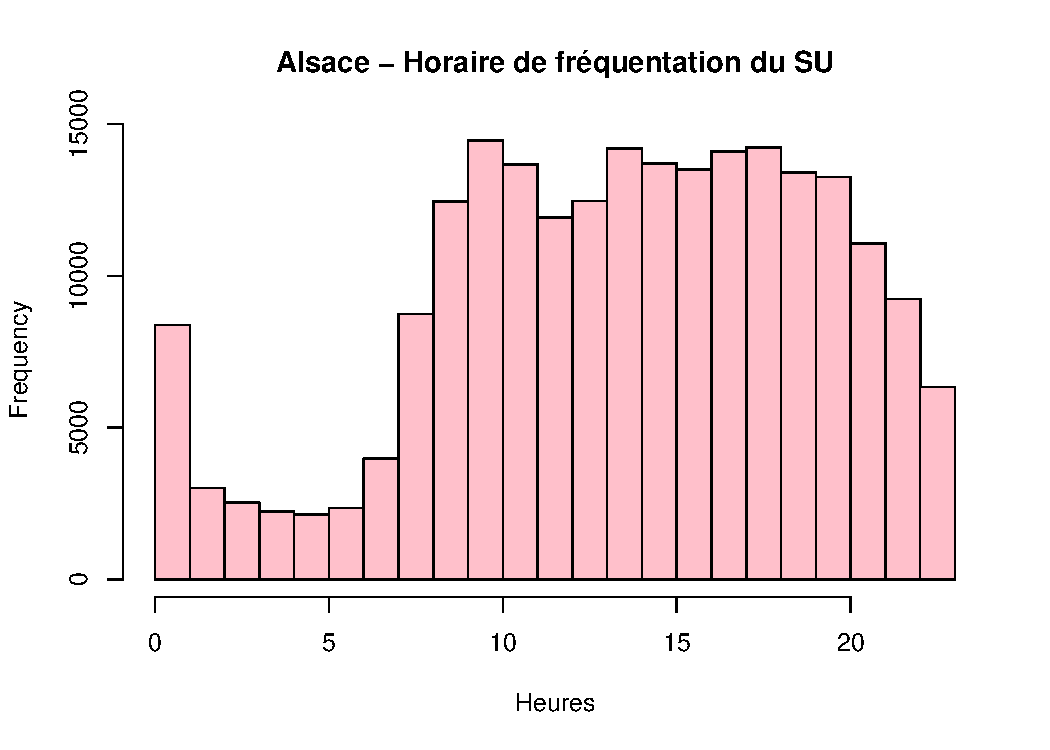
\includegraphics[width=\maxwidth]{figure/test23} 

\end{knitrout}

\end{center}
\caption{Horaires d'arrivée aux urgences en Alsace 2013}
\label{passage:als}
\end{figure}
%---------------------------------------------------------------------------- RADAR 1

\begin{figure}
\begin{center}
\begin{knitrout}
\definecolor{shadecolor}{rgb}{0.969, 0.969, 0.969}\color{fgcolor}
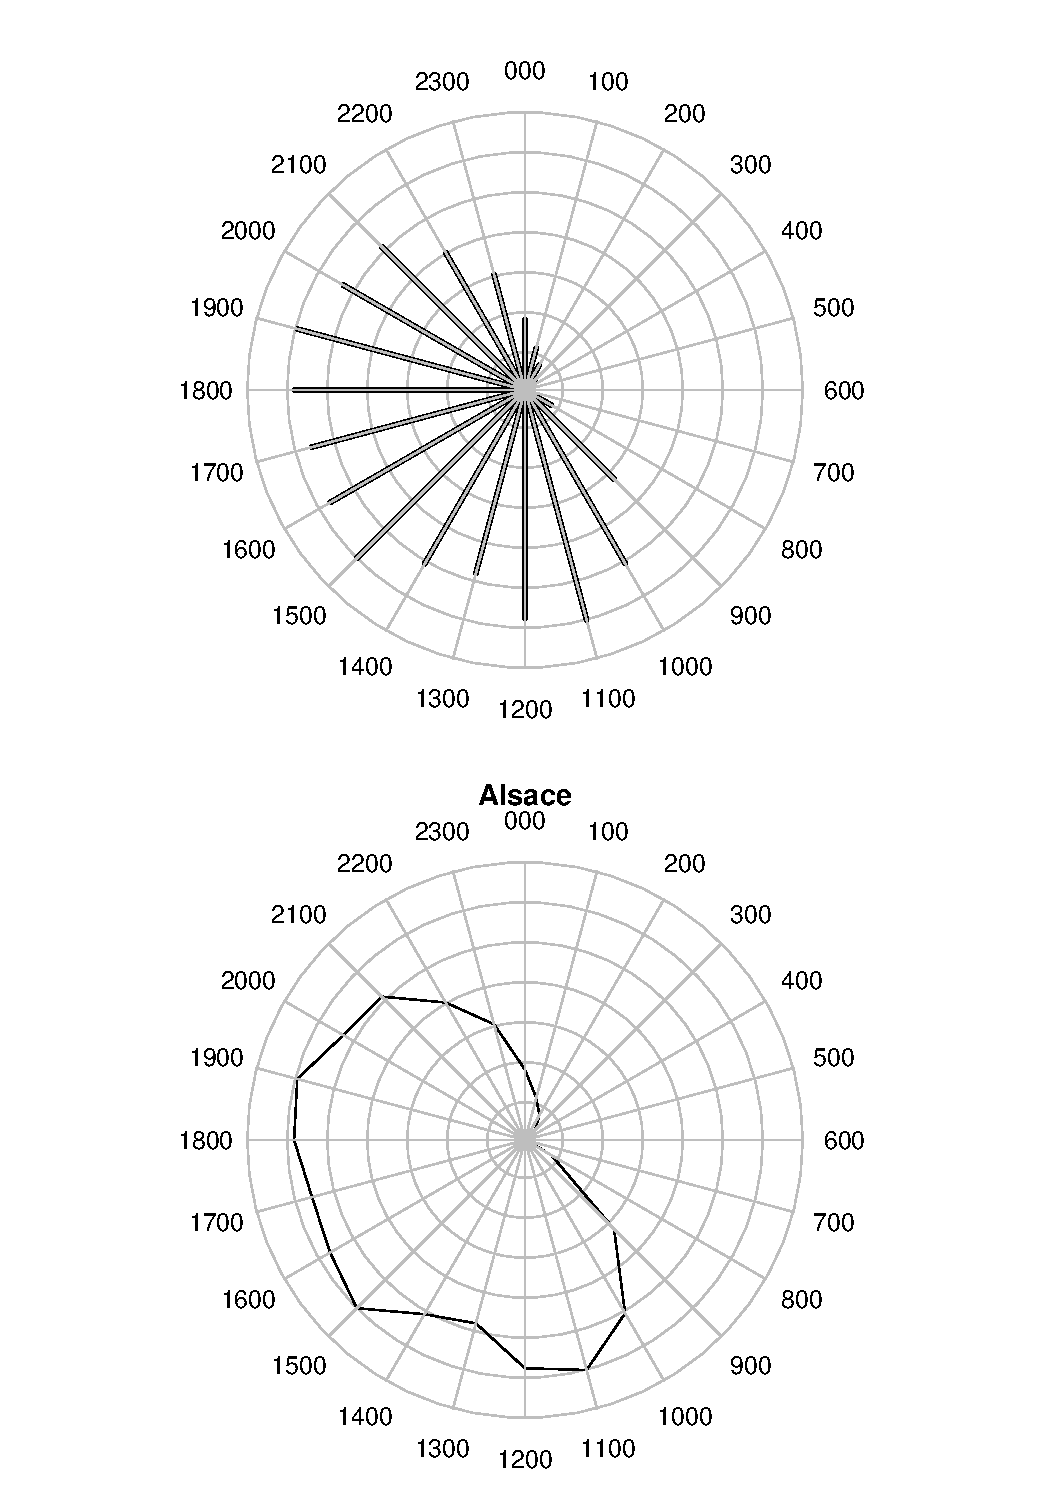
\includegraphics[width=\maxwidth]{figure/test25} 

\end{knitrout}

\end{center}
\caption{Horaires d'arrivée aux urgences en Alsace 2013}
\label{radar:als}
\end{figure}

%---------------------------------------------------------Radar HUS
\begin{figure}
\begin{center}
\begin{knitrout}
\definecolor{shadecolor}{rgb}{0.969, 0.969, 0.969}\color{fgcolor}
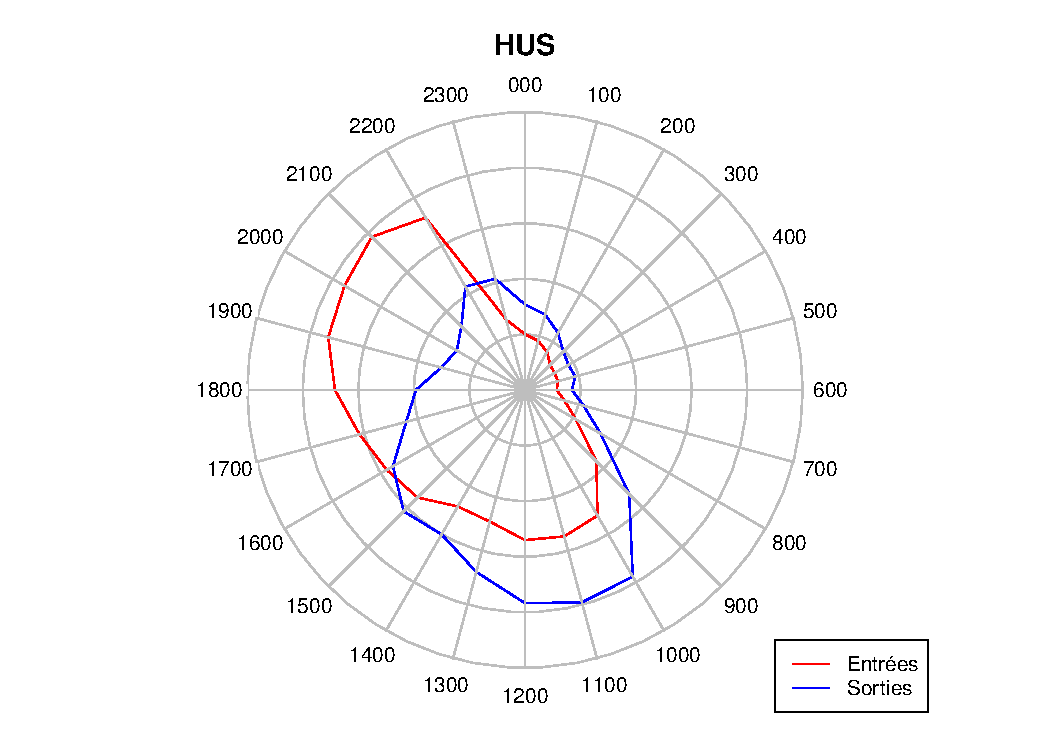
\includegraphics[width=\maxwidth]{figure/test2} 

\end{knitrout}

\end{center}
\caption{HUS: répartition des arrivées et départs aux urgences}
\label{passage:hus}
\end{figure}

%----------------------------------------------------------------
\begin{figure}
\begin{center}
\begin{knitrout}
\definecolor{shadecolor}{rgb}{0.969, 0.969, 0.969}\color{fgcolor}
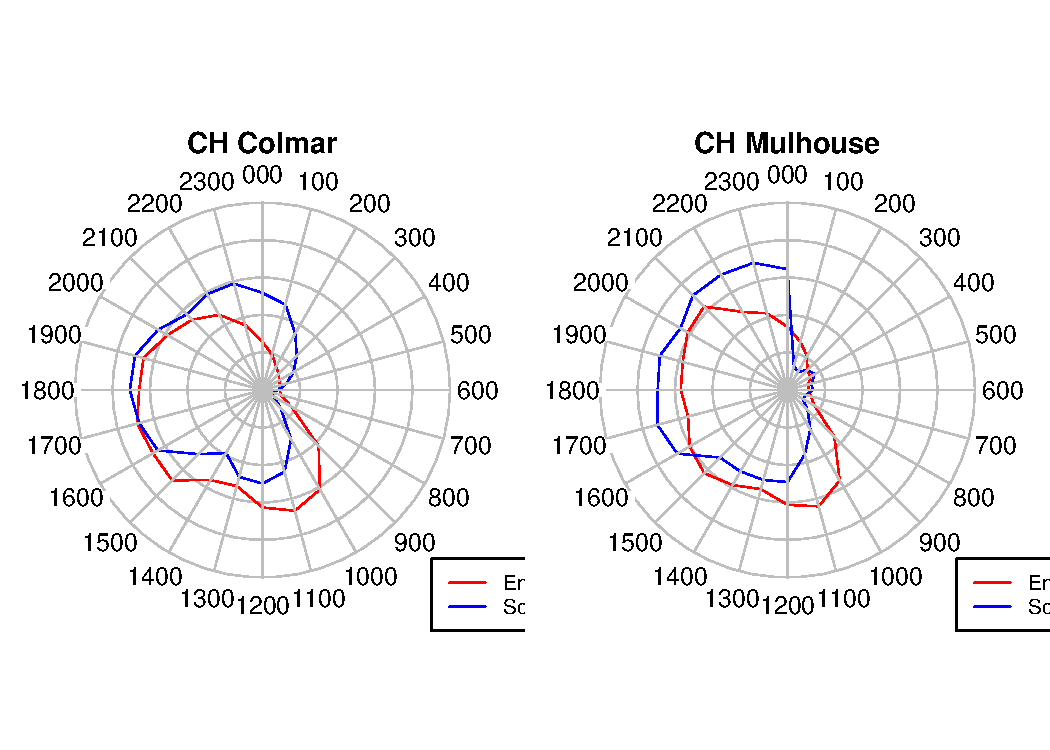
\includegraphics[width=\maxwidth]{figure/test22} 

\end{knitrout}

\end{center}
\caption{CH Colmar et Mulhouse: répartition des arrivées et départs aux urgences}
\label{passage:col}
\end{figure}



\subsection*{Passages par tranches d'âge}

\chapter{Modalité d'admission}
\section*{Origine des patients}
\section*{Mode de transport}
\section*{Origine géographique}

\chapter{Durée de passage}
\section*{Selon l'heure}
\section*{Selon l'âge}
\section*{Selon le jour de la semaine}
\section*{Selon la structure}
\subsection*{Pourcentage de passages en moins de 4 heures par établissement}
\section*{Selon l'orientation}
\section*{Selon la gravité}

\chapter{Codage diagnostic}

\chapter{Modalités de sortie}

% sortie.Rnw

Le RPU connaît trois mode de sortie des urgences:
\begin{enumerate}
  \item le décès
  \item le retour à domicile (ou ce qui en tient lieu)
  \item l'hospitalisation
\end{enumerate}
Cependant la réalité est plus complexe

La destination de concerne que les patients qui ont été hospitalisés.

\begin{itemize}
  \item NA:    Pas d'informations
  \item MCO:		Hospitalisation conventionnelle
  \item SSR:		Soins de suite et de réadaptation
  \item SLD:		Soins de longue durée
  \item PSY: 		Psychiatrie
  \item HAD:		Hospitalisation à domicile
  \item HMS:		Hébergement médico-social
\end{itemize}

\begin{knitrout}
\definecolor{shadecolor}{rgb}{0.969, 0.969, 0.969}\color{fgcolor}\begin{kframe}


{\ttfamily\noindent\bfseries\color{errorcolor}{\#\# Error: replacement has 0 rows, data has 105979}}\begin{verbatim}
## character(0)
## <0 x 0 matrix>
\end{verbatim}
\end{kframe}
\end{knitrout}



\chapter{Modalités d'orientation}

\chapter{Courbes d'activité régionale}
\section*{Variation du nombre total de passages journaliers}
\section*{Variation du pourcentage journalier de retour à domicile}

%===================================================================== PARTIE 3
\part{Activité par service d'urgence}

\chapter{SAU des Hôpitaux universitaires}

% SuHus.Rnw
% Activité des SU des HUS
Les Hôpitaux universitaires de Strasbourg ont une offre étendue en matière d'urgences et seuleument certaines activités génèrent des RPU.
On compte:
\begin{enumerate}
  \item SU adulte du NHC
  \item SU adulte de HTP
  \item SU pédiatrique de HTP
  \item SU SOS mains (CCOM)
  \item SU Gynéco-obstétrique à HTP
\end{enumerate}
Auxquels il faut rajouter les services assurant un accueil des urgences 24h/24h et qui ne transitent pas par les SU. Ce sont les correspondants privilégiés du SAMU 67 et des transporteurs sanitaires (ASSU, VSAV, SMUR):
\begin{enumerate}
  \item Réanimations médicales de HTP et NHC
  \item Réanimations chirurgicales de HTP et NHC
  \item Réanimation pédiatrique polyvalente de HTP
  \item Unité neuro-vasculaire (HTP)
  \item SI cardio-vasculaire (NHC)
\end{enumerate}

\section{Activité globale}




Entre le 2013-01-01 00:11:00 et le 2013-04-30 23:56:00, 13095 RPU ont été transmis, alors que 41561 dossiers ont été déclarés au serveur régional. 
1, 1, 1, 1, 1



%===================================================================== PARTIE 4
\part{Activité des SAMU d'Alsace}

\chapter{Test un}

%\SweaveOpts{concordance=TRUE}
\begin{itemize}
  \item test2.Rnw exemple de graphiques avec label
\end{itemize}

\begin{knitrout}
\definecolor{shadecolor}{rgb}{0.969, 0.969, 0.969}\color{fgcolor}\begin{kframe}
\begin{alltt}
n <- \hlfunctioncall{dim}(d1)
\hlfunctioncall{print}(n)
\end{alltt}
\begin{verbatim}
## [1] 105979     20
\end{verbatim}
\begin{alltt}
\hlfunctioncall{names}(d1)
\end{alltt}
\begin{verbatim}
##  [1] "id"            "CODE_POSTAL"   "COMMUNE"       "DESTINATION"  
##  [5] "DP"            "ENTREE"        "EXTRACT"       "FINESS"       
##  [9] "GRAVITE"       "MODE_ENTREE"   "MODE_SORTIE"   "MOTIF"        
## [13] "NAISSANCE"     "ORIENTATION"   "PROVENANCE"    "SEXE"         
## [17] "SORTIE"        "TRANSPORT"     "TRANSPORT_PEC" "AGE"
\end{verbatim}
\end{kframe}
\end{knitrout}



\chapter{test deux}
\begin{knitrout}
\definecolor{shadecolor}{rgb}{0.969, 0.969, 0.969}\color{fgcolor}\begin{kframe}
\begin{alltt}

\hlfunctioncall{str}(d1)
\end{alltt}
\begin{verbatim}
## 'data.frame':	105979 obs. of  20 variables:
##  $ id           : chr  "2c9d83843bf5e01d013bf5e985d20225" "2c9d83843bf5e01d013bf5e986950226" "2c9d83843bf5e01d013bf5e987620227" "2c9d83843bf5e01d013bf5e988060228" ...
##  $ CODE_POSTAL  : Factor w/ 1277 levels "00000","00159",..: 706 706 706 706 706 701 818 706 706 706 ...
##  $ COMMUNE      : Factor w/ 2691 levels "00","01257 DRESDEN ALLEMAGNE",..: 2184 2184 2184 2184 741 2048 2033 2184 2184 2184 ...
##  $ DESTINATION  : Factor w/ 7 levels "NA","MCO","SSR",..: NA NA NA NA NA NA 2 NA 2 NA ...
##  $ DP           : chr  "R104" "J038" "S617" "M485" ...
##  $ ENTREE       : chr  "2013-01-01 00:04:00" "2013-01-01 00:16:00" "2013-01-01 00:26:00" "2013-01-01 00:32:00" ...
##  $ EXTRACT      : chr  "2013-01-01 05:37:00" "2013-01-01 05:37:00" "2013-01-01 05:37:00" "2013-01-01 05:37:00" ...
##  $ FINESS       : Factor w/ 11 levels "3Fr","Alk","Col",..: 10 10 10 10 10 10 10 10 10 10 ...
##  $ GRAVITE      : Factor w/ 7 levels "1","2","3","4",..: 2 2 3 2 2 1 3 2 2 2 ...
##  $ MODE_ENTREE  : Factor w/ 4 levels "NA","Mutation",..: 4 4 4 4 4 4 4 4 4 4 ...
##  $ MODE_SORTIE  : Factor w/ 5 levels "NA","Mutation",..: 4 4 4 4 4 4 2 4 2 4 ...
##  $ MOTIF        : chr  "GASTRO04" "DIVERS23" "TRAUMATO10" "TRAUMATO02" ...
##  $ NAISSANCE    : chr  "1960-04-08 00:00:00" "1986-03-05 00:00:00" "1971-12-22 00:00:00" "1927-04-27 00:00:00" ...
##  $ ORIENTATION  : Factor w/ 13 levels "CHIR","FUGUE",..: NA NA NA NA NA NA 5 NA 5 NA ...
##  $ PROVENANCE   : Factor w/ 7 levels "NA","MCO","SSR",..: 6 6 6 6 6 6 6 6 6 6 ...
##  $ SEXE         : Factor w/ 3 levels "F","I","M": 3 3 3 1 3 3 1 1 1 1 ...
##  $ SORTIE       : chr  "2013-01-01 02:38:00" "2013-01-01 00:38:00" "2013-01-01 02:07:00" "2013-01-01 01:52:00" ...
##  $ TRANSPORT    : Factor w/ 6 levels "AMBU","FO","HELI",..: 4 4 4 1 4 4 6 6 4 4 ...
##  $ TRANSPORT_PEC: Factor w/ 3 levels "AUCUN","MED",..: 1 1 1 3 1 1 2 2 1 1 ...
##  $ AGE          : num  52 26 41 85 39 9 79 50 46 18 ...
\end{verbatim}
\begin{alltt}
\hlfunctioncall{summary}(d1)
\end{alltt}
\begin{verbatim}
##       id             CODE_POSTAL           COMMUNE       DESTINATION   
##  Length:105979      68000  : 7771   MULHOUSE   :12389   MCO    :23062  
##  Class :character   68200  : 6557   STRASBOURG :11504   PSY    :  399  
##  Mode  :character   68100  : 5866   COLMAR     : 7768   SSR    :   17  
##                     67100  : 5129   HAGUENAU   : 2267   HMS    :    8  
##                     67000  : 3757   SELESTAT   : 2000   SLD    :    4  
##                     67600  : 3005   SAINT LOUIS: 1817   (Other):    0  
##                     (Other):73894   (Other)    :68234   NA's   :82489  
##       DP               ENTREE            EXTRACT              FINESS     
##  Length:105979      Length:105979      Length:105979      Col    :21841  
##  Class :character   Class :character   Class :character   Mul    :16790  
##  Mode  :character   Mode  :character   Mode  :character   Hus    :13095  
##                                                           Hag    :11627  
##                                                           Sel    : 9685  
##                                                           Dia    : 9605  
##                                                           (Other):23336  
##     GRAVITE         MODE_ENTREE       MODE_SORTIE       MOTIF          
##  2      :64451   NA       :    0   NA       :    0   Length:105979     
##  3      :12856   Mutation : 1282   Mutation :21950   Class :character  
##  1      :12797   Transfert: 1128   Transfert: 1523   Mode  :character  
##  4      : 1320   Domicile :91250   Domicile :66755                     
##  P      :  480   NA's     :12319   Décès    :    0                     
##  (Other):  284                     NA's     :15751                     
##  NA's   :13791                                                         
##   NAISSANCE          ORIENTATION      PROVENANCE    SEXE     
##  Length:105979      UHCD   :11496   PEA    :59352   F:50853  
##  Class :character   MED    : 5662   PEO    : 9254   I:    1  
##  Mode  :character   CHIR   : 2342   MCO    : 2574   M:55125  
##                     PSA    :  954   SSR    :   11            
##                     SI     :  445   PSY    :   11            
##                     (Other): 1481   (Other):    9            
##                     NA's   :83599   NA's   :34768            
##     SORTIE          TRANSPORT     TRANSPORT_PEC        AGE     
##  Length:105979      AMBU :16290   AUCUN  :75794   Min.   :  0  
##  Class :character   FO   :  508   MED    : 2120   1st Qu.: 18  
##  Mode  :character   HELI :   37   PARAMED: 2430   Median : 39  
##                     PERSO:58281   NA's   :25635   Mean   : 41  
##                     SMUR : 1027                   3rd Qu.: 63  
##                     VSAB : 9263                   Max.   :112  
##                     NA's :20573                   NA's   :5
\end{verbatim}
\end{kframe}
\end{knitrout}


\index{test}
\index{Eclipse@Eclipse!solaire}
\index{Orbite!périgée@périgée}
test biblio \cite{1}
%===================================================================== PARTIE 5
\part{Annexes}
\appendix
\chapter{Méthodologie}

% methodologie.Rnw

\section*{Taux de passage aux urgences}
  \begin{displaymath}
    \frac{\text{Nombre de passages déclarés par les SU}}{\text{Population globale d'Alsace}}
  \end{displaymath}

\section*{Taux de recours aux urgences}
\begin{displaymath}
    \frac{\text{Nombre de passages d' Alsace}}{\text{Population globale d'Alsace}}
  \end{displaymath}
Le Nombre de passages d' Alsace est la somme des passages dans les SU alsacien ET des passages de résidents alsacien dans des SU limitrophes.

\section*{Taux d'intervention régional}
\begin{displaymath}
    \frac{\text{Nombre de patients pris en charge par les SMUR d'Alsace quelque soit le code postal du lieu d'intervention}}{\text{Population globale d'Alsace}}
  \end{displaymath}

\section*{Taux de recours régional}
\begin{displaymath}
    \frac{\text{Nombre de patients pris en charge par un SMUR dont l'intervention a lieu sur le territoire régional }}{\text{Population globale d'Alsace}}
  \end{displaymath}

\section*{Rapport de masculinité ou sex-ratio}
\begin{displaymath}
    \frac{\text{Nombre d'Hommes}}{\text{Nombre de Femmes}} \times 100
\end{displaymath}

Une valeur supérieure à 1 indique qu'il y a plus d'hommes que de femmes.

\section*{Définition de la semaine}
La semaine est définie comme la péride complémentaire du week-end. La semaine s'étend du lundi $08:00$ heures au vendredi $19:59$.

\section*{Définition du Week-end}
L'offre de soins comme la fréquentation des SU n'est pas identique en coiurs de semaine et en fin de semaine. C'est pourquoi est introduite la notion temporelle de week-end.
Le week-end est défini comme la période allant du vendredi soir 20h au lundi matin 07h59.

\section*{Moyenne mobile}
Une moyenne mobile permet de lisser une série de valeurs, permettant de gommer des fluctuations temporelles. La moyenne mobile d'odre $7$ est très utilisée pour analyser les données temporelles. Elle permet notamment d'atténuer les pics de fréquentation des SU le week-end.
\begin{displaymath}
    \frac{\text{somme des passages 7 jours consécutifs}}{7}
\end{displaymath}
Les moyennes mobiles sont généralement présentées sous forme "glissante", c'est à dire sous la forme d'une succession de groupe de sept éléments, décalés d'une journée.

\section*{Pondération annuelle et mensuelle}
Le nombre de jour dans un mois est variable d'un mois à l'autre. Il en va de même pour le nombre de jours d'une année, où du nombre de répétitions d'un jour donné de la semaine.

\chapter{Glossaire}

% glossaire.Rnw

\glossary{AIT Accident (Vasculaire) Ischemique Transitoire}



\subsection*{AIT}
\index{AIT}
Accident (Vasculaire) Ischemique Transitoire

\subsection*{ANTARES}
\index{ANTARES}
Adaptation Nationale des Trasmissions Aux Risques Et Secours

\subsection*{AR}
\index{AR}
Ambulance de Réanimation (voir UMH)

\subsection*{ARS}
\index{ARS}
Agence Régionale de Santé

\subsection*{AVC}
\index{Accident Vasculaire Cérébral}

cellule régionale d’appui et de pilotage sanitaire (CRAPS)
service zonal de défense et de sécurité (SZDS)
plateforme de veille et d’urgence sanitaire (PVUS)
cellule zonale d’appui (CZA). Structure de crise de l’ARS de zone, elle est constituée autour du SZDS qui assure une fonction de coordination en collaboration étroite avec la/les CRAPS activée(s) en ARS.
Directeur général de la santé (DGS) ou le Haut fonctionnaire de défense et de sécurité (HFDS)
Centre de crise sanitaire (CCS
Centre opérationnel zonal renforcé (COZ-R) de l’état-major interministériel de zone de défense et de sécurité (EMIZDS).
Système d’information sanitaire des alertes et crises (SISAC) de la DGS.




\chapter{RPU}
\chapter{Bibliographie}
\bibliography{../../rpu}
\chapter{Index}
\printindex
\end{document}
